\documentclass[12pt]{article}
\usepackage[utf8]{inputenc}
\usepackage[T1]{fontenc}
\usepackage{csvsimple}
\usepackage{booktabs}
\usepackage{siunitx}
\usepackage{float}
\usepackage[margin=0.5in]{geometry}
\usepackage{graphicx}
\usepackage{pgfplots}
\usepackage{tikz}

\newcommand{\distplot}[4]{
\begin{tikzpicture}
\begin{axis}[
height = 70,
width = 0.8\textwidth,
xbar stacked,
axis y line = none,
axis x line = none,
xmin = 0,
nodes near coords,
every node near coord/.append style={yshift=10pt},
]
\addplot coordinates {(#1,0)};
\addplot coordinates {(#2,0)};
\addplot coordinates {(#3,0)};
\addplot coordinates {(#4,0)};
\end{axis}
\end{tikzpicture}
}

\newcommand{\distplotlegend}[4]{
\begin{tikzpicture}
\begin{axis}[
height = 70,
width = 0.8\textwidth,
xbar stacked,
axis y line = none,
axis x line = none,
xmin = 0,
nodes near coords,
every node near coord/.append style={yshift=10pt},
legend style={at={(0.5,-0.1)},anchor=north,draw=none,column sep=1ex,},
legend columns=-1
]
\addplot coordinates {(#1,0)};
\addplot coordinates {(#2,0)};
\addplot coordinates {(#3,0)};
\addplot coordinates {(#4,0)};
\addlegendentry{Safe};
\addlegendentry{Borderline};
\addlegendentry{Rare};
\addlegendentry{Outlier};
\end{axis}
\end{tikzpicture}
}

\pgfplotsset{compat=1.15}
\graphicspath{ {./images/} }
\usetikzlibrary{arrows,decorations.markings}

\title{Types of Examples - nonOrdinal}

\begin{document}

\section{Imbalance}

In real world classification problems, class imbalance is a common occurrence. For example, in medical data, patients suffering from some condition are usually a minority compared to the group not affected by it. Imbalanced data has a negative impact on classifier learning process. Most often, when training on imbalanced data, resulting model is biased in favour for the larger class. Extensive reaserch has been carried out in order to understand the problem and find ways to reduce it \cite{Napierala2016, Blaszczynski2014}. Sampling methods, as well as learning algorithms were proposed. Sampling methods can be divided into over-sampling or under-sampling techniques, adding artificial examples to minority class or removing examples from majority class respectively. Algorithms used on imbalanced data are usually ensambles -- classifiers consisting of multiple models trained on different data subsets.

The source of imbalance, however, is not always the data itself. Class imbalance may be caused by the procedures used for classifier training. In case of a multiclass classification problem, a typical approach is to reduce it to a number of binary subproblems. This allows to use algorithms designed for binary classification. Making such transformation may, however, create imbalance. Figure \ref{img:balanced} shows an example artificial dataset. The data consists of examples described by two numeric features and divided into three classes. There is $150$ examples in each class.

\begin{figure}[H]
\centering
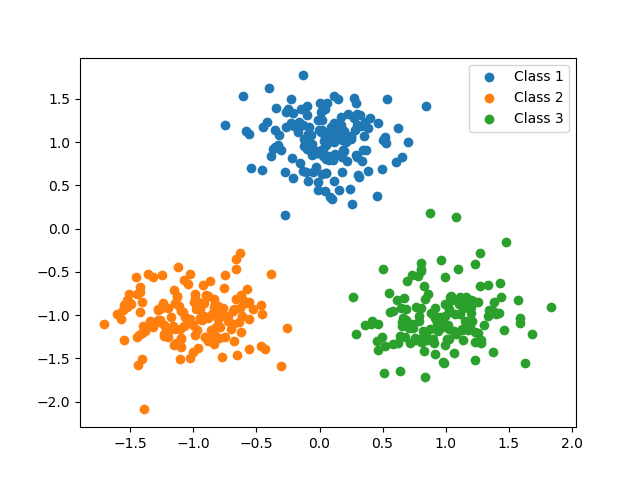
\includegraphics[width=0.6\textwidth]{balanced_data.png}
\caption{Balanced multiclass dataset}
\label{img:balanced}
\end{figure}

In a typical one-vs-rest approach, the problem could be reduced to $3$ binary subproblems. In this case, the training data for each subproblem is imbalanced with imabalance ratio being $1:2$. Despite the dataset having all of the classes equally numerous, one-vs-rest algorithm leads to class imbalance appearing in subproblems training data.

It is also possible for the classes in a multiclass problem to be ordered. In such case, reduction into binary subproblems can be made with regards to the order. A typical approach involves grouping the data into unions. For example, an equally distributed four-class problem would be transformed as shown in Figure \ref{img:balanced_ordered}. Classes in this problem are ordered, with class $Cl_1$ being the worst and $Cl_4$ the best.

\begin{figure}[H]
\centering
\begin{tikzpicture}
\draw (0,0) -- (8,0);
\node at (1,-0.6) {$Cl_1$};
\draw (2,0.5) -- (2,-0.5);
\node at (3,-0.6) {$Cl_2$};
\draw (4,0.5) -- (4,-0.5);
\node at (5,-0.6) {$Cl_3$};
\draw (6,0.5) -- (6,-0.5);
\node at (7,-0.6) {$Cl_4$};
\draw [decoration={markings,mark=at position 1 with
    {\arrow[scale=3,>=stealth]{>}}},postaction={decorate}] (4,-1) -- (4,-3);
\end{tikzpicture}

\begin{tikzpicture}
\draw (0,0) -- (8,0);
\node at (1,-0.6) {$Cl_1^\leq$};
\draw (2,0.5) -- (2,-0.5);
\node at (5,-0.6) {$Cl_2^\geq$};
\end{tikzpicture}

\begin{tikzpicture}
\draw (0,0) -- (8,0);
\node at (2,-0.6) {$Cl_2^\leq$};
\draw (4,0.5) -- (4,-0.5);
\node at (6,-0.6) {$Cl_3^\geq$};
\end{tikzpicture}

\begin{tikzpicture}
\draw (0,0) -- (8,0);
\node at (3,-0.6) {$Cl_3^\leq$};
\draw (6,0.5) -- (6,-0.5);
\node at (7,-0.6) {$Cl_4^\geq$};
\end{tikzpicture}
\caption{Ordered multiclass dataset transformation}
\label{img:balanced_ordered}
\end{figure}

Dividing the dataset in this case also causes imbalance. It is worth noting, however, that class imbalance appears when unions border moves closer to the best or the worst class. When the border is placed in the middle -- unions are balanced.

In both of the above examples, classes consist of the same number of examples. Such artificial datasets show how imbalance may be caused by the procedures used. In real-world datasets equal distributions are rarely the case. It is therefore the combination of data characteristics and procedures used that influences the imbalance.

\section{Types of minority examples}

In \cite{Napierala2016} a learning example assesment method was introduced. It was designed to estimate learning difficulty for minority class examples in binary classification problem. In order to analyze datasets in this study, a modified version of the method was implemented based on the description in \cite{Napierala2016}. Modifications included data transformation which allowed the method to be used for ordered multiclass datasets.

Originally, the method takes a binary dataset as input. Examples of the minority class are labelled with one of the four types: Safe, Borderline, Rare, Outlier. For a multiclass dataset, transformation methods were implemented to transform the data into a number of binary subsets. Example type classification was then performed on each of the binary subsets and the results were then aggregated to construct the final output for multiclass data. Two transformation methods were introduced.

\subsection{Union vs. union transformation}

The first transformation method is a standard approach visualized in Figure \ref{img:balanced_ordered}. In general case, $n - 1$ binary sets are made for a dataset with $n$ classes. For each class $Cl_t$, where $t \in \{1, n-1\}$ the original dataset is divided into  an upward union $Cl_{t + 1}^\geq$ and downward union $Cl_{t}^\leq$.

\subsection{Class vs. union transformation}

The other method divides the original data into subsets consisting of a class and an union. Figure \ref{img:subset} visualizes the divide for an imaginary four-class dataset using this transformation.

\begin{figure}[H]
\centering
\begin{tikzpicture}
\draw (0,0) -- (8,0);
\node at (1,-0.6) {$Cl_1$};
\draw (2,0.5) -- (2,-0.5);
\node at (3,-0.6) {$Cl_2$};
\draw (4,0.5) -- (4,-0.5);
\node at (5,-0.6) {$Cl_3$};
\draw (6,0.5) -- (6,-0.5);
\node at (7,-0.6) {$Cl_4$};
\draw [decoration={markings,mark=at position 1 with
    {\arrow[scale=3,>=stealth]{>}}},postaction={decorate}] (4,-1) -- (4,-3);
\node at (4,-3) {};
\end{tikzpicture}

\begin{tikzpicture}
\draw (0,0) -- (4,0);
\draw[dotted] (4,0) -- (8,0);
\node at (1,-0.6) {$Cl_1^\leq$};
\draw (2,0.5) -- (2,-0.5);
\node at (3,-0.6) {$Cl_2$};
\draw (4,0.5) -- (4,-0.5);
\end{tikzpicture}

\begin{tikzpicture}
\draw[dotted] (0,0) -- (2,0);
\draw (2,0) -- (8,0);
\draw (2,0.5) -- (2,-0.5);
\node at (3,-0.6) {$Cl_2$};
\draw (4,0.5) -- (4,-0.5);
\node at (6,-0.6) {$Cl_3^\geq$};
\end{tikzpicture}

\begin{tikzpicture}
\draw (0,0) -- (6,0);
\draw[dotted] (6,0) -- (8,0);
\node at (2,-0.6) {$Cl_2^\leq$};
\draw (4,0.5) -- (4,-0.5);
\node at (5,-0.6) {$Cl_3$};
\draw (6,0.5) -- (6,-0.5);
\end{tikzpicture}

\begin{tikzpicture}
\draw[dotted] (0,0) -- (4,0);
\draw (4,0) -- (8,0);
\draw (4,0.5) -- (4,-0.5);
\node at (5,-0.6) {$Cl_3$};
\draw (6,0.5) -- (6,-0.5);
\node at (7,-0.6) {$Cl_4^\geq$};
\end{tikzpicture}

\caption{Class vs. union transformation}
\label{img:subset}
\end{figure}

In general case, a dataset consisting of $n$ classes is split into $(n-2)*2$ subsets. This method should therefore be applied to datasets with the class number higher than $2$. In contrary to the previous transformation, subsets do not contain all of the examples. Dotted lines in the schema above mark areas not included in a given subset.

\subsection{Neighbourhood types}

Example type classification is performed on the basis of a classified example's neighbourhood. The number of the same class examples is compared to the number of opposing class examples. The type is determined by the ratio of these two amounts. Two methods for choosing the neighbourhood were introduced.

\subsubsection{K-Nearest Neighbours}

The first method is based on the kNN algorithm. Given an example from the dataset and a distance metric, the neighbourhood is defined as $k$ nearest examples with regards to the metric. HVDM, introduced in \cite{Wilson1997}, was used as a metric. It allows to measure distance between examples described by both numeric and nominal attributes. $K$ is a parameter, with $5$ being the default value.

\subsubsection{Kernel function}

The second method also utilizes HVDM. In this case, all examples with distance to classified example smaller than a given value, are selected as neighbours. The limiting value, called \textit{kernel width}, is a method parameter.

\section{Binary classification datasets}

Before applying learning difficulty assesment method to multiclass problems, some experiments from \cite{Napierala2016} were replicated in order to verify if own implementation is correct. The same binary classification datasets from UCI repository were used, parameters of the method were also set to be the same as in the original study. A union vs. union comparison was used, which on a binary dataset causes the modified method to behave exactly as the original in \cite{Napierala2016}.

\subsection{KNN analysis}

In Tables \ref{tab:knn_own} and \ref{tab:knn_org} own and original results are presented. Table \ref{tab:knn_diff} contains differences between corresponding positions. In this experiment, kNN neighbourhood function with $k=5$ was used.

\newcolumntype{H}{S[round-mode=places,round-precision=2]}

\begin{table}[H]
\begin{minipage}[t]{0.5\textwidth}
\centering
\csvreader[
    separator=semicolon,
    tabular=lHHHH,
    respect underscore,
    head to column names,
    separator=semicolon,
    table head=\toprule Dataset & S\% & B\% & R\% & O\% \\ \midrule,
    table foot=\bottomrule
]{../results/percentage/nonOrdinal/real/union_vs_union_knn.csv}
{}
{\texttt{\name} & \safe & \borderline & \rare & \outlier}
\caption{Union vs. union - KNN}
\label{tab:knn_own}
\end{minipage}
\begin{minipage}[t]{0.5\textwidth}
\centering
\begin{tabular}{lrrrr}
    \toprule
    Dataset & S\% & B\% & R\% & O\% \\ \midrule
    \texttt{abalone} & $8.36$ & $20.60$ & $20.60$ & $50.45$ \\
    \texttt{breast-cancer} & $24.71$ & $25.88$ & $32.94$ & $16.47$ \\
    \texttt{car} & $47.83$ & $39.13$ & $8.70$ & $4.35$ \\
    \texttt{cleveland} & & $31.43$ & $17.14$ & $51.43$ \\
    \texttt{cmc} & $17.72$ & $44.44$ & $18.32$ & $19.52$ \\
    \texttt{ecoli} & $28.57$ & $54.29$ & $2.86$ & $14.29$ \\
    \texttt{haberman} & $4.94$ & $61.73$ & $18.52$ & $14.81$ \\
    \texttt{hepatitis} & $15.63$ & $62.50$ & $6.25$ & $15.63$ \\
    \texttt{scrotal-pain} & $38.98$ & $45.76$ & $10.17$ & $5.08$ \\
    \texttt{solar-flare} & & $48.84$ & $11.63$ & $39.53$ \\
    \texttt{transfusion} & $18.54$ & $47.19$ & $11.24$ & $23.03$ \\
    \texttt{vehicle} & $74.37$ & $24.63$ & & $1.01$ \\
    \texttt{yeast} & $5.88$ & $47.06$ & $7.84$ & $39.22$ \\
    \bottomrule
\end{tabular}
\caption{Original -- KNN}
\label{tab:knn_org}
\end{minipage}
\begin{minipage}{0.5\textwidth}
\centering
\begin{tabular}{lrrrr}
    \toprule
    Dataset & S\% & B\% & R\% & O\% \\ \midrule
    \texttt{abalone} & $0.3$ & $1.5$ & $1.19$ & $0$\\
    \texttt{breast-cancer} & $1.18$ & $1.18$ & $1.18$ & $1.18$ \\
    \texttt{car} & $0$ & $0$ & $0$ & $0$ \\
    \texttt{cleveland} & $0$ & $5.72$ & $5.72$ & $0$ \\
    \texttt{cmc} & $0$ & $3.3$ & $3.3$ & $0$ \\
    \texttt{ecoli} & $0$ & $2.86$ & $2.85$ & $0$ \\
    \texttt{haberman} & $0$ & $4.94$ & $4.94$ & $0$ \\
    \texttt{hepatitis} & $21.87$ & $21.87$ & $0$ & $0$ \\
    \texttt{scrotal-pain} & $0$ & $1.69$ & $1.69$ & $0$ \\
    \texttt{solar-flare} & $0$ & $2.33$ & $2.32$ & $0$ \\
    \texttt{transfusion} & $0$ & $5.06$ & $5.05$ & $0$ \\
    \texttt{vehicle} & $0$ & $0.51$ & $0.5$ & $0$ \\
    \texttt{yeast} & $0$ & $3.92$ & $3.92$ & $0$ \\
    \bottomrule
\end{tabular}
\caption{Difference -- KNN}
\label{tab:knn_diff}
\end{minipage}
\end{table}

Minor differences are visible, however, overall tendencies appear the same. In case of \texttt{car} dataset, results do not differ at all. On the other hand, Safe and Borderline percantage for \texttt{hepatitis} show roughly a $20\%$ misalignment. Differences may have appeared due to data preprocessing. Examples with missing values were deleted from datasets used in this study. It is not known if the data in the original study was also preprocessed and if so, what methods were used. For majority of the datasets, difference appears for Borderline and Rare percentage and has equal value. This may indicate that majority of the differences is caused by Borderline examples being classified as Rare or vice-versa. Some implementation differences are possible and in case of distinction between Rare and Borderline, additional conditions may have been applied in the original study.
\subsection{Kernel analysis}

Similar verification experiment was carried out using kernel neighbourhood. Thresholds for classification were set as described in the original study. Kernel width was set to average distance between minority examples and their $5$ nearest neughbours in a given dataset. Results are presented in Table \ref{tab:kernel_own}. Table \ref{tab:kernel_org} shows reference results, differences are shown in Table \ref{tab:kernel_diff}.

\begin{table}[H]
\begin{minipage}[t]{0.5\textwidth}
\centering
\csvreader[
    separator=semicolon,
    tabular=lHHHH,
    respect underscore,
    head to column names,
    separator=semicolon,
    table head=\toprule Dataset & S\% & B\% & R\% & O\% \\ \midrule,
    table foot=\bottomrule
]{../results/percentage/nonOrdinal/real/union_vs_union_kernel.csv}
{}
{\texttt{\name} & \safe & \borderline & \rare & \outlier}
\caption{Union vs. union -- Kernel}
\label{tab:kernel_own}
\end{minipage}
\begin{minipage}[t]{0.5\textwidth}
\centering
\begin{tabular}{lrrrr}
    \toprule
    Dataset & S\% & B\% & R\% & O\% \\ \midrule
    \texttt{abalone} & $7.8$ & $23.7$ & $11.4$ & $57.1$ \\
    \texttt{breast-cancer} & $18.8$ & $46.3$ & $33.8$ & $1.3$ \\
    \texttt{car} & $47.8$ & $43.5$ & $8.7$ & \\
    \texttt{cleveland} & $6.7$ & $30.0$ & $13.3$ & $50.0$ \\
    \texttt{cmc} & $17.2$ & $44.3$ & $10.4$ & $28.2$ \\
    \texttt{ecoli} & $25.8$ & $61.3$ & $3.2$ & $9.7$ \\
    \texttt{haberman} & $15.1$ & $56.2$ & $16.4$ & $12.3$ \\
    \texttt{hepatitis} & $13.6$ & $63.6$ & $9.1$ & $13.6$ \\
    \texttt{scrotal-pain} & $24.4$ & $53.3$ & $11.1$ & $11.1$ \\
    \texttt{solar-flare} & $7.1$ & $45.2$ & $7.1$ & $40.5$ \\
    \texttt{transfusion} & $15.1$ & $57.8$ & $9.6$ & $17.5$ \\
    \texttt{vehicle} & $77.4$ & $18.9$ & & $3.7$ \\
    \texttt{yeast} & $15.2$ & $37.0$ & $2.2$ & $45.7$ \\
    \bottomrule
\end{tabular}
\caption{Original -- Kernel}
\label{tab:kernel_org}
\end{minipage}
\begin{minipage}[t]{0.5\textwidth}
\centering
\begin{tabular}{lrrrr}
    \toprule
    Dataset & S\% & B\% & R\% & O\% \\ \midrule
    \texttt{abalone} & $3.02$ & $12.66$ & $22.93$ & $7.25$ \\
    \texttt{breast-cancer} & $4.68$ & $15.71$ & $7.38$ & $12.82$ \\
    \texttt{car} & $26.11$ & $43.5$ & $8.7$ & $26.09$ \\
    \texttt{cleveland} & $0.95$ & $12.86$ & $12.41$ & $1.43$ \\
    \texttt{cmc} & $2.79$ & $11.57$ & $8.22$ & $6.03$ \\
    \texttt{ecoli} & $0.09$ & $15.59$ & $5.37$ & $10.3$ \\
    \texttt{haberman} & $3.99$ & $36.45$ & $28.04$ & $12.39$ \\
    \texttt{hepatitis} & $17.65$ & $41.72$ & $15.9$ & $8.28$ \\
    \texttt{scrotal-pain} & $9.15$ & $16.01$ & $2.46$ & $22.8$ \\
    \texttt{solar-flare} & $0.12$ & $24.27$ & $9.18$ & $15.31$ \\
    \texttt{transfusion} & $4.99$ & $15.67$ & $15.12$ & $5.53$ \\
    \texttt{vehicle} & $12.07$ & $3.21$ & $3.52$ & $5.35$ \\
    \texttt{yeast} & $3.44$ & $11.51$ & $11.53$ & $3.32$ \\
    \bottomrule
\end{tabular}
\caption{Difference -- Kernel}
\label{tab:kernel_diff}
\end{minipage}
\end{table}

In this case, more significant differences are visible, but overall tendencies still match. The only concern might be caused by the results received for \texttt{car} dataset. In case of kNN variant of the method, results for this dataset were completely aligned with those received in \cite{Napierala2016}. It might indicate that this data is identical to the one used in the original study. Since the results received using kernel method are clearly different, own implementation of this neighbourhood function most probably differs from the original. Potential differences could lie for example in the way Epanechnikov function is utilized to estimate probability or how kernel width is set.

\subsection{Artificial datasets}

To further verify the method, the same experiment was carried out on artificially created datasets. The goal was to study the differences of own implementation of kNN and kernel method. The results are presented in Tables \ref{tab:gen_union_knn} and \ref{tab:gen_union_kernel}. Table \ref{tab:knn_kernel_diff} shows differences.

\begin{table}[H]
\begin{minipage}{0.5\textwidth}
\fontsize{10pt}{12pt}\selectfont
\centering
\csvreader[
    separator=semicolon,
    tabular=lHHHH,
    respect underscore,
    head to column names,
    separator=semicolon,
    table head=\toprule Dataset & S\% & B\% & R\% & O\% \\ \midrule,
    table foot=\bottomrule
]{../results/percentage/nonOrdinal/gen/union_vs_union_knn.csv}
{}
{\texttt{\name} & \safe & \borderline & \rare & \outlier}
\caption{Union vs. union -- KNN}
\label{tab:gen_union_knn}
\end{minipage}
\begin{minipage}{0.5\textwidth}
\fontsize{10pt}{12pt}\selectfont
\centering
\csvreader[
    separator=semicolon,
    tabular=lHHHH,
    respect underscore,
    head to column names,
    separator=semicolon,
    table head=\toprule Dataset & S\% & B\% & R\% & O\% \\ \midrule,
    table foot=\bottomrule
]{../results/percentage/nonOrdinal/gen/union_vs_union_kernel.csv}
{}
{\texttt{\name} & \safe & \borderline & \rare & \outlier}
\caption{Union vs. union -- Kernel}
\label{tab:gen_union_kernel}
\end{minipage}
\begin{minipage}{0.5\textwidth}
\fontsize{10pt}{12pt}\selectfont
\centering
\begin{tabular}{lrrrr}
    \toprule
    Dataset & S\% & B\% & R\% & O\% \\ \midrule
    \texttt{flower5-3d-10-20-35-35} & $7.45$ & $20.74$ & $13.3$ & $0$ \\
    \texttt{flower5-3d-100-0-0-0} & $0.53$ & $2.13$ & $1.06$ & $1.6$ \\
    \texttt{flower5-3d-30-40-15-15} & $3.73$ & $10.64$ & $14.36$ & $0$ \\
    \texttt{flower5-3d-30-70-0-0} & $0$ & $3.2$ & $0$ & $3.19$ \\
    \texttt{flower5-3d-50-50-0-0} & $0.54$ & $1.06$ & $0.53$ & $1.06$ \\
    \texttt{paw3-3d-10-20-35-35} & $1.34$ & $4$ & $2.67$ & $0$ \\
    \texttt{paw3-3d-100-0-0-0} & $0$ & $0$ & $0$ & $0$ \\
    \texttt{paw3-3d-30-40-15-15} & $2$ & $6$ & $8.66$ & $0.67$ \\
    \texttt{paw3-3d-30-70-0-0} & $6.67$ & $2$ & $2$ & $6.67$ \\
    \texttt{paw3-3d-50-50-0-0} & $2$ & $1.34$ & $2.67$ & $0.67$ \\
    \bottomrule
\end{tabular}
\caption{Difference -- KNN, Kernel}
\label{tab:knn_kernel_diff}
\end{minipage}
\end{table}

Distributions of the example types received by both kNN and kernel method are similar. The most significant difference was observed for 'flower5-3d-10-20-35-35' dataset, where Borderline percentage in case of kernel method was about $20\%$ higher. It is worth remembering that kernel variant of the method is not expected to return exactly the same results as kNN. While kNN neighbourhood always maintains the same size, kernel function allows the number of neighbours to differ between separate classifications. It varies depending on the density of classified example's neighbourhood and is therefore more responsive. In case of exceptionally dense or sparse neighbourhoods, kNN function may be prone to errors due to arbitrary selection of a fixed number of neighbours. Kernel method takes into account a more significant sample. 

Based on all of the above observations, own implementation of the method is assumed to be correct.

\section{Ordinal datasets analysis}

Selected ordinal datasets were analysed using the implemented method. The goal of the analysis was to gain overall insight into the data and, more importatly, to verify how introducing order of the classes affects the problem in terms of learning difficulty. 

$15$ datasets were selected. In each case an order of the output classes was defined. Results were aggregated into a single distribution per dataset. Combining two variants of neighbourhood (kNN, kernel) with two dataset reduction methods (union vs. union, class vs. union) led to four setups. Standard parameters were used ($k=5$, kernel width set to mean distance to $5$ nearest neighbours of minority examples). Results for each setup are presented in Tables \ref{tab:ordinal_union_knn} to \ref{tab:ordinal_class_kernel}. In case of binary datasets, class vs. union variant was not used. 

\begin{table}[H]
\begin{minipage}{0.5\textwidth}
\fontsize{10pt}{12pt}\selectfont
\centering
\csvreader[
    separator=semicolon,
    tabular=lHHHH,
    respect underscore,
    head to column names,
    separator=semicolon,
    table head=\toprule Dataset & S\% & B\% & R\% & O\% \\ \midrule,
    table foot=\bottomrule
]{../results/percentage/ordinal/union_vs_union_knn.csv}
{}
{\texttt{\name} & \safe & \borderline & \rare & \outlier}
\caption{Union vs. union - KNN}
\label{tab:ordinal_union_knn}
\end{minipage}
\begin{minipage}{0.5\textwidth}
\fontsize{10pt}{12pt}\selectfont
\centering
\csvreader[
    separator=semicolon,
    tabular=lHHHH,
    respect underscore,
    head to column names,
    separator=semicolon,
    table head=\toprule Dataset & S\% & B\% & R\% & O\% \\ \midrule,
    table foot=\bottomrule
]{../results/percentage/ordinal/class_vs_union_knn.csv}
{}
{\texttt{\name} & \safe & \borderline & \rare & \outlier}
\caption{Class vs. union -- KNN}
\label{tab:ordinal_class_knn}
\end{minipage}
\begin{minipage}{0.5\textwidth}
\fontsize{10pt}{12pt}\selectfont
\centering
\csvreader[
    separator=semicolon,
    tabular=lHHHH,
    respect underscore,
    head to column names,
    separator=semicolon,
    table head=\toprule Dataset & S\% & B\% & R\% & O\% \\ \midrule,
    table foot=\bottomrule
]{../results/percentage/ordinal/union_vs_union_kernel.csv}
{}
{\texttt{\name} & \safe & \borderline & \rare & \outlier}
\caption{Union vs. union - Kernel}
\label{tab:ordinal_union_kernel}
\end{minipage}
\begin{minipage}{0.5\textwidth}
\fontsize{10pt}{12pt}\selectfont
\centering
\csvreader[
    separator=semicolon,
    tabular=lHHHH,
    respect underscore,
    head to column names,
    separator=semicolon,
    table head=\toprule Dataset & S\% & B\% & R\% & O\% \\ \midrule,
    table foot=\bottomrule
]{../results/percentage/ordinal/class_vs_union_kernel.csv}
{}
{\texttt{\name} & \safe & \borderline & \rare & \outlier}
\caption{Class vs. union -- Kernel}
\label{tab:ordinal_class_kernel}
\end{minipage}
\end{table}

Confronting results for union-vs-union divide with results for class-vs-union divide provides an insight on how introducing more information about classes order affects learning difficulty. Tables \ref{tab:ordinal_union_knn} and \ref{tab:ordinal_class_knn} respectively, provide this comparison for kNN neighbourhood function. In most cases, after introducing more order information, a shift towards unsafe examples is visible. The most significant increases are present in Borderline and Rare percentages. Veryfying results for kernel neighbourhood, however, reveals that the shift is not so transparent. In case of 'Car', 'Dataset3',  'ESL', 'Housing', 'LEV' and 'SWD' datasets a slight increase in Safe percantage can be noticed. On the other hand, 'Balance Scale' and 'ERA' datasets were drastically shifted into $100\%$ Outlier distribution. This may lead to a conslusion that in some cases, a multiclass problem might become significantly more difficult because  of introducing classes order. 

Even further insight can be gained by analyzing results aggregated per division. Tables \ref{tab:3_union_kernel} and \ref{tab:3_class_kernel} show numbers of examples labelled as given minority type in every division made on 'Dataset 3'. Classes in this dataset belong to $\{1, 2,3, 4, 5\}$.

\begin{table}[H]
\fontsize{10pt}{12pt}\selectfont
\centering
\begin{tabular}[t]{lllr}
\toprule
Union (min) & Union (maj) &  & Total \\ 
\midrule
$\leq 1$ & $\geq 2$ & \distplot{107}{69}{15}{52} & 243 \\ 
$\leq 2$ & $\geq 3$ & \distplot{241}{108}{4}{186} & 539 \\ 
$\geq 4$ & $\leq 3$ & \distplot{246}{54}{3}{129} & 432 \\ 
$\geq 5$ & $\leq 4$ & \distplotlegend{25}{43}{20}{36} & 124 \\
\bottomrule
\end{tabular}
\caption{\texttt{dataset3} -- Union vs. union, kernel}
\label{tab:3_union_kernel}
\end{table}

\begin{table}[H]
\fontsize{10pt}{12pt}\selectfont
\centering
\begin{tabular}[t]{lllr}
\toprule
Class & Union &  & Total \\ 
\midrule
$2$ & $\leq 1$ & \distplot{187}{35}{2}{72} & 296 \\ 
$2$ & $\geq 3$ & \distplot{152}{68}{4}{72} & 296 \\ 
$3$ & $\leq 2$ & \distplot{221}{34}{3}{99} & 357 \\ 
$3$ & $\geq 4$ & \distplot{192}{62}{4}{99} & 357 \\ 
$4$ & $\leq 3$ & \distplot{189}{35}{4}{80} & 308 \\ 
$4$ & $\geq 5$ & \distplotlegend{215}{11}{2}{80} & 308 \\ 
\bottomrule
\end{tabular}
\caption{\texttt{dataset3} -- Class vs. union, kernel}
\label{tab:3_class_kernel}
\end{table}

This dataset appears shifted towards safe examples after introducing class-vs-union division. Part of the reason for this is that minority class has changed for some divisions. For union-vs-union comparison, union of 'at most class 1', consisting only of class '1', was a minority compared to union of 'at least class 2'. In this case, $110$ examples were classified as safe, but a total of $133$ examples constituted for unsafe examples. However, the same classes border, when compared using class-vs-union method becomes 'safer'. When class '2' is considered minority, and union 'at most class 1'  a majority, $203$ examples were classified safe and $93$ unsafe.

Yet another meaningful conclusion can be drawn from detailed distributions. Tables \ref{tab:swd_union_kernel} and \ref{tab:swd_class_kernel} show the same comparison for 'SWD' dataset. Classes in this dataset belong to $\{2, 3, 4, 5\}$. Again, minority class changes depending on division method. For classes '2' and '3', an extreme imbalance appears. Union 'at most class 2' (only class '2') consists of a total of $33$ examples while class '3' accounts for $352$ examples. The same border from a class-vs-union perspective appears 'safer' due to scale difference.

Imbalance in datasets leads to higher learning difficulty. It is a widely discussed issue and many techniques were designed to address it. In case of ordered multiclass problem, the data is not the only source of imbalance. In fact, both division methods may infer it, since unions created in both procedures include different numbers of examples depending on how close the union border is to the best or worst class in range.

\begin{table}[H]
\fontsize{10pt}{12pt}\selectfont
\centering
\begin{tabular}[t]{lllr}
\toprule
Union (min) & Union (maj) &  & Total \\ 
\midrule
$\leq 2$ & $\geq 3$ & \distplot{5}{8}{10}{9} & 32 \\ 
$\leq 3$ & $\geq 4$ & \distplot{171}{133}{52}{28} & 384 \\ 
$\geq 5$ & $\leq 4$ & \distplotlegend{56}{106}{38}{17} & 217 \\ 
\bottomrule
\end{tabular}
\caption{\texttt{SWD} -- Union vs. union, kernel}
\label{tab:swd_union_kernel}
\end{table}

\begin{table}[H]
\fontsize{10pt}{12pt}\selectfont
\centering
\begin{tabular}[t]{lllr}
\toprule
Class & Union &  & Total \\ 
\midrule
$3$ & $\leq 2$ & \distplot{294}{32}{0}{26} & 352 \\ 
$3$ & $\geq 4$ & \distplot{155}{119}{50}{28} & 352 \\ 
$4$ & $\leq 3$ & \distplot{180}{173}{29}{17} & 399 \\ 
$4$ & $\geq 5$ & \distplotlegend{227}{133}{26}{13} & 399 \\ 
\bottomrule
\end{tabular}
\caption{\texttt{SWD} -- Class vs. union, kernel}
\label{tab:swd_class_kernel}
\end{table}


\bibliographystyle{unsrt}
\bibliography{sources}

\end{document}
